\documentclass{article}
\usepackage[utf8]{inputenc}
\usepackage[russian]{babel}
\usepackage{marginnote}
\usepackage{graphicx}
\usepackage{float}

\title{Базы данных, лекция 9}
\author{@mikhirurg}
\date{April 2020}

\begin{document}

\maketitle

\section{Безопасность и защита информации}

\begin{itemize}
    \item Надежность и безопасность БД? СУБД? ИС?
    \newline 
    \item Что такое безопасная система?
    \newline Что такое безопасная система (Trusted Computer System Evaluation Criteria "The Orange Book" 1985). 
    \newline Книга о безопасности информационных систем.
    \begin{figure}[H]
    \centering
    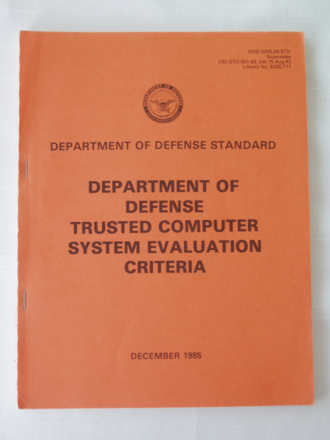
\includegraphics[width = .5\linewidth]{img0}
    \caption{Trusted Computer System Evaluation Criteria}
  \end{figure}
    CRUD — акроним, обозначающий четыре базовые функции, используемые при работе с базами данных: создание (англ. create), чтение (read), модификация (update), удаление (delete).
    \item Иерархия уровней безопасности:  
    \begin{itemize}
        \item \textbf{Класс D} - Система не соответствует другим классам
        \item \textbf{Класс C} - Есть индентификация, аутентификация, учет событий и дискреционный контроль доступа.
        \item \textbf{Класс B} - Мандатное управление доступом
        \item \textbf{Класс A} - Проверенный дизайн
    \end{itemize}
\end{itemize}

\subsection{Системы класса C}
\begin{itemize}
    \item Идентификация, классификация индентификаторов: 
    \begin{itemize}
        \item То, что знает субъект
        \newline \textit{Пароль, пин-код, девичья фамилия матери, имя домашнего животного и тд.}
        \item То, что принадлежит субъекту
        \newline \textit{Смарт-карта, мобильный телефон, любой объект, принадлежащий субъекту.}
        \item То, что является неотъемлимой характеристикой субъекта.
        \newline \textit{Биометрия, цифровой почерк.}
    \end{itemize}
    \item Аутентификация, многофакторная аутентификация.
\end{itemize}

\begin{itemize}
    \item Авторизация, дискреционный контроль доступа
    \newline
    \newline
    \begin{tabular}{|c|c|c|c|}
        \hline
        & Объект1 & ... & ОбъектM\\
        \hline
        Субъект1 & Read, modify, delete & ... & read, change, delegate access \\ 
        \hline
        ... & ... & ... & ... \\  
        \hline
        СубъектN & Read & ... & Read, access to..    \\
        \hline
    \end{tabular}
    \end{itemize}
    Метод определения дискреционногго доступа
    \begin{itemize}
        \item Суперпользователем
        \item Владельцем
        \item Делегированием своего доступа (плохо и ненадежно)
    \end{itemize}
    
    \subsubsection{Подклассы систем класса C}
    
    \begin{itemize}
        \item \textbf{Подкласс C1} Разделение пользователей и данных, контур обеспечения безопасности, 
        дискреционное управление доступом.
        \newline \textbf{Доступ к объектам имеет изолированная доверенная база.}
        \item \textbf{Подкласс C2} Доступ через процедуру авторизации, журнал контроля доступа к системе, изоляция ресурсов.
        \newline \textit{Выделяя память, мы должны быть уверены, что её нельзя проанализировать и получить доступ к информации, обрабатываемой другим процессом ранее.}
    \end{itemize}
    
    \subsection{Системы Класса B}
    Системы мандатного управления доступом.
    \textit{\newline То есть для того, что бы получивший доступ субъект не мог нарушить конфеденциальность доступность данных используется мандатный доступ с помощью меток доступа.}
    \newline'Жесткое' Правило:
    \begin{itemize}
        \item Чтение своего уровня и ниже
        \item Запись на свой уровень и уровень выше
    \end{itemize}
    
    \subsubsection{Подклассы класса B}
    
    \begin{itemize}
        \item \textbf{Подкласс B1} - Мандатное управление доступа к выбранным субъектам и объектам, изоляция процессов. 
        \item \textbf{Подкласс B2} - Структурированная защита - применение мандатного управления ко всем объектами субъектам, отдельный защищенный способ первичной индентификации и аутентификации, модульная структура контура безопасности.
        \item \textbf{Подкласс B3} Домены безопасности - выделенный администратор системы безопасности, мониторинг обращений
    \end{itemize}
    
    \subsection{Системы класса A}
    \begin{itemize}
        \item Формализированные процедуры проектирования
        \item Формализированные процедуры упревления
        \item Формализированные процедуры распространения 
    \end{itemize}
    
    \subsection{Ролевая модель доступа}
    \begin{itemize}
        \item Преимущества
        \begin{itemize}
            \item Сокращение операции назначения и проверки прав доступа
            \item Централизация управления
        \end{itemize}
        \item Типовые роли 
        \begin{itemize}
            \item Администратор СУБД
            \item Админ БД
            \item Привелегированный пользователь
            \item Обычный пользователь
        \end{itemize}
    \end{itemize}
    
    \subsection{Аудит безопасности}
    
    \textbf{Протоколирование}
    \newlineЗаписывать каждую попытку аутентификации не очень удобно, так как это потредует большого расхоба памяти + обрабатывать огромные логи долго.
    \newline \textbf{Выборочное протоколирование} - записываем каждую n-ую попытку входа.
    \newline \textbf{Адаптивное протоколирование} - запись попыток в записимости от некоторого условия.
    
    \subsection{Шифрование баз данных}
    \begin{itemize}
        \item Прозрачное шифрование 
        \item Column-level encryption - Шифрование на уровне столбцов. Удобно разделять доступ к разным столбцам.
        \item Шифрование файловой системы.
        \newline удобно исспользовать в распределённых системах
        \item Шифрование на уровне приложений
        \newline База данных не занимается шифрованием, это делают сами приложения.
        \newline Минус: невозможно адекватное индексирование по шифрованным данным
        \item Hashing - Хэширование - паролю пользователя сопоставляется результат некоторой хеш-функции.
    \end{itemize}
    
    Угроза действий привелегированных пользователей. 
    Решение проблемы:
    \begin{itemize}
        \item Резервное копирование
    \end{itemize}
    
\end{document}
